\chapter{To Sort}
\section{Spin}
The magnetic moment of elementary particles is called spin. 

% Dirac Equation 

% Pauli Equation 



\section{Zeeman Effect}\label{zeeman}
When no magnetic field is applied to a system, the magnetic dipoles of the orbital electron and spin have no preferred direction. 
The energy levels for all combinations of $L$ and $S$ (all $J$) are equivalent. 

If a magnetic field is applied the magnetic moments interact with that field via the \index{Zeeman!Zeeman interaction}. 
The \index{Zeeman!Zeeman effect} consists of atomic energy level splitting when an external magnetic field is imposed on a sample \cite{Nabokov2002}. 

The classical expression for the energy of a dipole in a magnetic field
\begin{equation}
    E = -\vec{\mu}\cdot\vec{B}
    \label{eq:}
\end{equation}
may be replaced with the Hamiltonian for a quantum mechanical system 
\begin{equation}
    \hat{H}_{\text{Zeeman}} = - \hat{\vec{\mu}}\cdot \vec{B}. 
    \label{eq:}
\end{equation}

The negative sign indicates that when the magnetic moment is parallel to the magnetic field the lowest energy is achieved. 

Thus distinct quantum systems with different $J$ and thus different projections of angular momentum ($m_J$) have different energies due to their interaction with a magnetic field. 

Considering a simple two-level system ($S=1/2$), the energy difference between the spin being aligned or anti-aligned with the field is called the Zeeman energy. 

The Hamiltonian to describe the energy is, using the total angular momentum form of \eqref{eq:orbital_magnetic_moment_operator_bohr_magneton_g_factor}, 
\begin{equation}
    \hat{H}_{\text{Zeeman}} = g \mu_B \hat{\vec{S}}\cdot\vec{B}. 
    \label{eq:}
\end{equation}

Without loss of generality we may direct the magnetic field along the $z$ axis and reduce the scalar product to only the $z$ component. Now, using $S=1/2$ quantised along the $z$ axis, i.e. $m_S = \pm 1/2$ we find the Zeeman energy by solving the Shr\"odinger equation 
\begin{equation}
    \hat{H}_{\text{Zeeman}} \ket{S, m_S} = E_{\text{Zeeman}}\ket{S, m_S} 
    % \label{eq:}
\end{equation}
which, to a factor is equivalent to, by \eqref{eq:zthcomponent}, to
\begin{equation}
    \hat{S}_{z} \ket{S, m_S} = m_S\ket{S, m_S}.
    % \label{eq:}
\end{equation}

Thus we find the two eigenvalues to be
$$E_+ =\frac{1}{2}g\mu_BB, \qquad E_-=-\frac{1}{2}g\mu_BB$$
and thus the Zeeman energy is given by $g\mu_B B$. 

The $S=1/2$ system is thus doubly \index{degenerate} and the \index{degeneracy} is lifted by the application a magnetic field. The Zeeman energy is the difference between the two states and it grows linearly with $B$. 

This may be generalised to a more complex system by considering the total angular momentum $J$ where the energy difference between states is given by 
\begin{equation}
   \Delta E = g_J \mu_B B. 
    \label{eq:zeeman_energy}
\end{equation}






\input{Sections/HahnEcho.tex}
%Dipole 
%Fermi Contact



\input{Sections/SpinBaths.tex}
\section{Spin-Orbit Interaction}
The orbital magnetic dipole may interact with the intrinsic spin magnetic dipole via the \index{spin-orbit interaction}{spin-orbit interaction}. This is represented by the spin-orbit Hamiltonian with $\lambda$ representing the constant of the coupling: 
\begin{equation}
    H_{\ce{SO}} = \lambda \hat{\vec{L}}\cdot\hat{\vec{S}}. 
    \label{eq:spin_orbit_hamiltonian}
\end{equation}

This is caused by the interaction between the magnetic field generated by the relativistic motion of the electron around the nucleus and that of the spin magnetic moment. The coupling is proportional to the atomic mass. 


\subsubsection{Extending to Quantum Mechanics}
Since the gyromagnetic ratio was calculated considering the motion of dipole in a loop, we may extend this to an electron in an orbit.

\begin{wrapfigure}{r}{0.5\textwidth}%
	% \centering%
	\begin{center}
		% 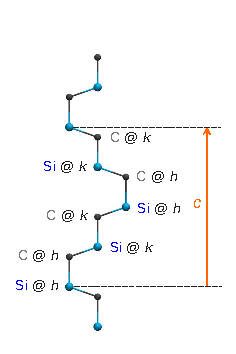
\includegraphics[width=0.38\textwidth]{figures/SiC-non-equiv-sites.pdf}%
		% MAGNETIC MOMENT ATOM
\begin{tikzpicture}[thick, scale=1.5]
  \def\rn{0.3}
  \def\re{0.15}
  \def\Rx{1.5}
  \def\Ry{0.5}
  %\draw[dashed] (-100:1.5*\rn) -- (80:1.5*\rn);
  \draw[dashed] (-\Rx,0) arc (180:0:{\Rx} and {\Ry});
  \draw[mu vector] (0,-1.8*\rn) -- (0,2.9*\rn) node[right] {$\vb*{\mu}$};
  \draw[charge+] (0,0) circle (\rn) node[scale=1.4] {+};
  \draw[dashed] (\Rx,0) arc (0:-180:{\Rx} and {\Ry});
  \draw[charge-]
    (-40:{\Rx} and {\Ry}) circle (\re) node[scale=0.8] {$-$}
    node[below right=0.2] {e};
  \draw[->]
    (-55:{1.15*\Rx} and {1.2*\Ry}) arc (-55:-72:{1.15*\Rx} and {1.2*\Ry});
  \draw[current]
    (-140:{1.15*\Rx} and {1.2*\Ry}) arc (-140:-100:{1.15*\Rx} and {1.2*\Ry})
    node[midway,below] {$I$};
\end{tikzpicture}

		\caption{Schematic of electron in orbit generating a magnetic moment.}%
	\end{center}
\end{wrapfigure}%
The fundamental change required to extend the model to quantum mechanics is the treatment of angular momentum which should now be quantised.
Thus, we replace our classical approximation of $\vec{G} = \vec{r} \times \vec{p}$ with the equation for the eigenvalues of the quantum mechanical representation of orbital angular momentum,
\begin{equation}
	\hat{G} = \hbar \hat{L}
	\label{eq:orbital_angular_momentum}
\end{equation}
where $\hat{L}$ is the operator of the orbital angular momentum (quantum number of orbital momentum).
The angular momentum and total energy are conserved in general in a closed system.

We consider the time independent \index{Shr\"odinger equation}{Shr\"odinger equation}
\begin{equation}
	\hat{H} \Psi_n = E_n \Psi_n
	\label{eq:TISE}
\end{equation}

and choose $\Psi_n$ such that it is an eigenfunction of the Hamiltonian, the total angular momentum squared ($L^2 = L_x^2 + L_y^2 + L_z^2$) and exactly one directional component of the angular momentum which is by convention chosen as $L_z$.

According to quantum mechanics the projection of $L$ along the \index{quantisation axis} ($m_L$) may take integer values $-L, -L + 1, \dots, L-1, L$.
Thus, we may describe a given quantum state by the angular momentum $L$ and it's projection $m_L$. Thus, using \index{Dirac notation}{Dirac Notation} we write
\begin{eqnarray}
	&\hat{H}\ket{L, m_L} &= E\ket{L, m_L} \\
	&\hat{L^2}\ket{L, m_L} &= L(L+1)\ket{L, M_L} \\
	&\hat{L_z}\ket{L, m_L} &= m_L\ket{L, m_L}. \label{eq:zthcomponent}
\end{eqnarray}
Thus, the operator which describes the orbital magnetic moment may be written using  \eqref{eq:gyromagnetic_ratio_electrons}, \eqref{eq:orbital_angular_momentum} as
\begin{equation}
	\hat{\vec{\mu}}_L = \gamma \hat{\vec{G}}_L = \gamma \hbar \hat{\vec{L}} = \frac{e\hbar}{2m_e c}\hat{\vec{L}}.
	\label{eq:orbital_magnetic_moment_operator}
\end{equation}

This leads to a quantity known as the \textbf{\index{Bohr magneton}{Bohr Magneton}}, $\mu_B$, given by \cite{Ramamurti1995-wg}
\begin{equation}
	\mu_B = \frac{|e|\hbar}{2m_e c}.
	\label{eq:bohr_magneton}
\end{equation}

Using this we may write \eqref{eq:orbital_magnetic_moment_operator} as
\begin{equation}
	\hat{\vec{\mu}}_L = -\mu_B\hat{\vec{L}}.
	\label{eq:orbital_magnetic_moment_operator_bohr_magneton}
\end{equation}


\subsection{g-factor}
The above expression is valid for the orbital electron but may be extended to a more general system by introducing a \index{g-factor}{g-factor}. The g-factor is equivalent to a dimensionless gyromagnetic ratio \cite{giancoli2008physics}, so \eqref{eq:orbital_magnetic_moment_operator_bohr_magneton} may be written with $g=1$ as
\begin{equation}
	\hat{\vec{\mu}}_L = -g\mu_B\hat{ \vec{L}}.
	\label{eq:orbital_magnetic_moment_operator_bohr_magneton_g_factor}
\end{equation}



\input{Sections/SpinCoupling.tex}
\section{Defect Orientation}

Colour centres or defects in general are part of the crystal lattice and thus have an associated orientation and direction within the lattice. This allows the definition of a \textbf{defect axis}. For example, in diamond the NV axis is defined as the vector from the vacancy towards the Nitrogen atom when the vacancy is taken as the origin of your co-ordinate system. 

In a tetragonal crystal, due to symmetry there are four possible orientations of a defect within the lattice: $111$, $1\overline{11}$, $\overline{1}1\overline{1}$ and $\overline{11}1$ directions. 

\section{Miller Indices}
The notation for defect orientation above is known as a Miller Index, and we consider the $111$ direction to be aligned with the defect axis. 

This means that if we know the orientation of our crystal then we can establish the orientations of the defect axis inside. For example, using a crystal for which all surfaces belong to the $\{001\}$ lattice planes, each surface normal is aligned with a Cartesian axis. Thus, by fixing the crystal in place, there remain just \textbf{four} possible angles which a defect axis can have with respect to the crystal surface.

Calculating the scalar product of any of the surface planar directions in the family of $\{001\}$ and the four possible orientations of the defect within the lattice we find $\cos\theta = \pm0.6$. Then, considering the physical solutions (from $0, 2\pi$) gives four possible angles that the (directed) defect axis may make with the surface of the crystal: $53.13^\circ$, $306.87^\circ$, $126.9^\circ$ and $233.13^\circ$ ($0.927$, $5.355$, $2.214$ and $4.069$ radians respectively). 






    


\input{Sections/SpinDetection.tex}
\input{Sections/SpinRelaxation.tex}
\input{Sections/DensityMatrices.tex}
\subsection{Magnetic Dipole}
Classically, the magnetic dipole is though of as a loop carrying an
electric current ($I$). 

The resultant \index{magnetic dipole moment}{magnetic dipole moment}, $\vec{\mu}$, is defined as the vector at a normal to the  
plane of the current loop, 
\begin{equation}
    \vec{\mu} = IS \vec{n}
    \label{eq:dipole_moment}
\end{equation}
where $I$ is the current in, and $S$ the surface area enclosed by, the loop. 

\begin{wrapfigure}{l}{0.4\textwidth}%
    \centering%
    % 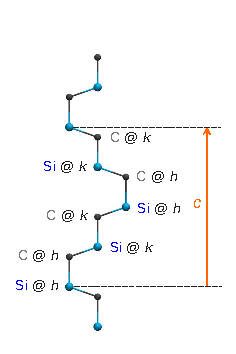
\includegraphics[width=0.38\textwidth]{figures/SiC-non-equiv-sites.pdf}%
        % B FIELD through current loop
\begin{tikzpicture}[scale=1.2, thick]
  \def\Rx{1.45}
  \def\Ry{0.43}
  \def\h{0.5}
  \def\H{3}
  \def\L{4}
  \def\NB{5}
  \def\ang{36}
  \coordinate (O) at (0,0);
  \coordinate (N) at (0,0.24*\H);
  \coordinate (M) at (0,0.45*\H);
  \coordinate (B) at (\ang:\H);
  
  % MAGNETIC FIELD
  \draw (-\Rx,0) arc (180:0:{\Rx} and {\Ry});
  \begin{scope}
    \clip ({-0.5*\L*cos(\ang)},-0.4*\H) rectangle ++({\L*cos(\ang)},\H);
    %\foreach \i [evaluate={\y=(\i-0.5)*\H/(\NB-0.5)/2;
    %                       \yl=-\H/2+(\i-0.5)*\H/(\NB-0.5)/2;}] in {1,...,\NB}{
    %  %\draw[BFieldLine,thin] (0,\y)++(\ang-180:0.5*\L) --++ (\ang:\L);
    %  %\draw[BFieldLine,thin] (0,-\y)++(\ang-180:0.5*\L) --++ (\ang:\L);
    %  \draw[BFieldLine,thin] (-\H/2,\y) -- ({-\H/2+(\H/2-\y)*cos(\ang)},\H/2);
    %  \draw[BFieldLine,thin] (-\H/2,-\y) -- ({-\H/2+(\H/2+\y)*cos(\ang)},+\H/2);
    %  \draw[BFieldLine,thin] ({\H/2-(\H/2+\yl)*cos(\ang)},-\H/2) -- (\H/2,\yl);
    %  \draw[BFieldLine,thin] ({\H/2-(\H/2-\yl)*cos(\ang)},-\H/2) -- (\H/2,-\yl);
    %}
    % \foreach \i [evaluate={\x=-0.31*\H+(\i-1)*0.62*\H/(\NB-1);
    %                        \y=-cot(\ang)*\x;
    %                        \a=0.50+0.017*\i}] in {1,...,\NB}{ %0.58-0.02*(\i-\NB/2-1)^2
    %   \draw[BFieldLine=\a] (\x,\y)++(\ang-180:\H) --++ (\ang:2*\H);
      %\fill[red] (\x,\y) circle (0.05);
    % }
  \end{scope}
  % \node[Bcol] at (\H/2,0.49*\H) {$\vb{B}$};
  
  % CIRCUIT
  \draw[white,very thick]
        (-\Rx,0) arc (-180:0:{\Rx} and {\Ry});
  \draw (-\Rx,0) arc (-180:0:{\Rx} and {\Ry});
  %\draw[white,very thick] (0,0) ellipse ({\R} and {0.3*\R});
  %\draw (0,0) ellipse ({\R} and {0.3*\R});
  %\draw (0,0) ellipse ({\R} and {0.3*\R});
  \draw[mu vector] (0,0) -- (M) node[above=-1, left=0] {$\vb*{\mu}$};
  \draw[vector] (0,0) -- (N) node[below=0,left=0] {$\vu{n}$};
  % \draw pic[->,"\small$\;\theta$",draw=black,angle radius=14,angle eccentricity=1.4]
    % {angle = B--O--N};
  \draw[white,very thick]
    (-150:{1.1*\Rx} and {1.16*\Ry}) arc (-150:-80:{1.1*\Rx} and {1.16*\Ry});
  \draw[current]
    (-135:{1.1*\Rx} and {1.16*\Ry}) arc (-135:-90:{1.1*\Rx} and {1.16*\Ry})
    node[midway,right=2,below] {$I$};
  
\end{tikzpicture}


  \caption{Schematic of current loop and induced magnetic moment.}%
\end{wrapfigure}%


The \index{magnetic dipole}{magnetic dipole} induces a magnetic field $\vec{B}$, which for points a large distance from the dipole may be calculated as \cite{Griffiths2012-pt}:
\begin{equation}
    \vec{B} = \frac{\mu_0}{4\pi} \frac{1}{r^3} \left[\frac{3(\vec{\mu} \cdot \vec{r}) \cdot \vec{r}}{r^2} - \vec{\mu}\right]
    \label{eq:}
\end{equation}

The symmetry of the field enables us to consider the direction of the dipole as aligned to the $z$-axis. Then, defining $x,y$ as usual by $r \cos\theta$ and $r \sin\theta$ respectively. We may decompose the \index{magnetic field}{magnetic field} in two separate components, parallel ($B_z$) and perpendicular ($B_x, B_y$): 
$$B_\parallel =\frac{\mu_0}{r^3}(3\cos^2 \theta - 1), \quad B_\perp = \frac{3\mu_0}{r^3}\cos\theta\sin\theta.$$
Where we use the Pythagorean principle to determine the overall magnitude $B = |\vec{B}|$ as
$$B = \sqrt{B_\parallel^2 + B_\perp^2}.$$

\input{Sections/RabiOscillations.tex}
\subsection{Gyromagnetic Ratio}
\subsubsection{Classical Derivation}
The current in equation \ref{eq:dipole_moment} is proportional to the angular momentum of the charge. That is, the dipole moment is always associated with an angular momentum $\vec{G} = \vec{r} \times \vec{p}$ with $\vec{r}$ the radius and $\vec{p}$ the momentum. 

Dividing the magnetic dipole moment by the angular momentum we find the \textbf{gyromagnetic ratio}. 
\begin{equation}
    \gamma = \frac{\vec{\mu}}{\vec{G}}.
    \label{eq:gyromagnetic_ratio}
\end{equation}

Without loss of generality we may consider the most simple case which is where the magnetic dipole moment is parallel (or anti-parallel) to the angular momentum. Then we may consider the absolute values for the dipole moment and the angular momentum: 
\begin{equation}
    \mu = IS, \quad I = 
    % \underbrace{\frac{q}{2\pi R}}_{\rho \text{ (charge density)}}v,
    \frac{qv}{2\pi R},
    \quad S = \pi R^2 
    % \label{eq:}
\end{equation}
We substitute $I$ and $S$ to find 
\begin{equation}
    \mu = \frac{qvR}{2} 
    % \label{eq:}
\end{equation}
% which we substitute into our equation for the gyromagnetic ratio 
% \begin{equation}
%     \gamma = \frac{\frac{qvR}{2}}{\vec{G}}. 
%     \label{eq:789}
% \end{equation}
and further, we equate the angular momentum vector, using the model of a planar loop to 
\begin{equation}
   G= m_q v R 
    % \label{eq:}
\end{equation}
leaving 
\begin{equation}
    \gamma = \frac{q}{2m_q } . 
    % \label{eq:}
\end{equation}

We finally consider that we may represent the, currently unknown, charge and mass as a sum of electron charges and masses. 
\begin{equation}
    \gamma = \frac{q}{2m_q } = \frac{\cancel{N}e}{2\cancel{N} m_e} \implies \gamma = \frac{e}{2 m_e}
    \label{eq:gyromagnetic_ratio}
\end{equation}

We therefore find that the gyromagnetic ratio of the electron depends only on fundamental constants \cite{bromley2000quantum}.

%pg 329 
% https://www.google.co.uk/books/edition/_/7qCMUfwoQcAC?hl=en&gbpv=1&bsq=walter%20greiner%20theoretical%20physics



\input{Sections/SpinInitialisation.tex}
\section{Lattice Symmetry}
Tetragonal lattice has the $$



\chapter{Task}
\section{Brief}

I think, as a start can go through section 3.2.4 in the attached PhD thesis? In particular check in details how to diagonalise the NV centre spin S=1 Hamiltonian to get Eq. 3.31?
You could also do some python simulations to plot how the spin levels (i.e. the eigenvalues of the spin Hamiltonian) change with applied magnetic field.

Once we've learned this, we can apply it to other spin defects in SiC.

\section{Work}
\subsection{Concepts and Nomenclature}
\subsubsection{Spin-Spin Interactions}
\subsubsection{Zeeman Splitting}
\subsubsection{Hyperfine Interaction}
\subsection{System Hamiltonian}\label{system_hamiltonian}
The ground state of the $\ce{NV^-}$ spin system in diamond is a triplet state, thus a $S=1$ system. 

The corresponding Hamiltonian, which it seems can be generalised to an electron spin system of a defect, can be expressed as: 
\begin{equation}
    H_{\ce{NV}} = H_{\ce{D}} + H_{\ce{Zeeman}} + H_{\ce{HF}} 
    \label{eq:nv_hamil}
\end{equation}

Here the labels $\ce{D}$, $\ce{Z}$ and $\ce{HF}$ describe the electron spin-spin interactions, the Zeeman interaction with an external magnetic field and the hyperfine interaction between the nuclparallel spin $I$ and the electron spin $S$ of the NV. 

They have the following forms: 
\begin{eqnarray}
    H_{\ce{D}} &=& D S_z^2 + E(S_x^2 + S_y^2) \label{H_D} \\
    H_{\ce{Z}} &=& g \mu_B \sum_{j}^{x,y,z} B_j \cdot S_j \label{H_Z} \\
    H_{\ce{HF}} &=& \vec{S} \cdot A \cdot \vec{I}. \label{H_HF}
\end{eqnarray}

\subsubsection{Spin-Spin Interaction}


The $E$ and $D$ in equation \ref{H_D} the fine structure constants of the spin
system, describing the spin-spin interaction and $S_j$ the corresponding spin operators
in x,y and z-direction. 

D is non-zero in system with axis of threefold (or other manifold) symmetry. 
The symmetry or spin quantization axis points along the connection of the nitrogen
atom and vacancy forming the defect. In bulk diamond $D$ is around 2.87 GHz at room temperature.

The definiteness, orientation and magnitude of $D$ is thus dependent on the specific spin system being studied. 

E occurs when there is a distortion of the point group symmetry, for example strain or an electrical field. In bulk diamond $E$ is typically negligibly small but especially in NDs, $E$ can be of the order of several MHz. 

Thus, similarly, the value of $E$ is a characteristic of the nature of the distortion and 
the specifics of the spin system being studied. 

\subsubsection{Zeeman Interaction}

$B_j$ in equation \ref{H_Z} is the magnetic field along the $x$, $y$ and $z$ direction, $g$ is the $g$-factor of the vacancy and $\mu_B$ the Bohr-Magneton, a constant. 

It seems often the scaled parameter $g\mu_B$ is considered, for the $\ce{NV^-}$ system this is around $28\;\ce{ GHz T^{-1}}$, but again, will be a characteristic of the system being studied. 

\subsubsection{Hyperfine Interaction}

Equation $\ref{H_HF}$ related the nuclear spin to the electron spin via the hyperfine tensor $A$ which has the form 
\begin{equation}
    A = \begin{pmatrix}
        A_\perp & 0 & 0 \\ 
        0 & A_\perp & 0 \\ 
        0 & 0 & A_\parallel
    \end{pmatrix}.
    \label{eq:hyperfine_tensor}
\end{equation}

$A_\parallel$ and $A_\perp$ are the axial and non-axial hyperfine parameters which encode two different interactions. 

\paragraph{Fermi Contact Interaction.}
This interaction is calculated by 
\begin{equation}
    f_A = \frac{A_\parallel + 2 A_\perp}{3}.
    \label{eq:fermi_contact}
\end{equation}

\paragraph{Anisotropic Interaction.}
This interaction is found by considering both spins as magnetic dipoles is calculated by 
\begin{equation}
    d_A = \frac{A_\parallel - A_\perp}{3}.
    \label{eq:anisotropic}
\end{equation}

For the $\ce{NV^-}$ system in diamond specifically, using the values for $A_\parallel$ and $A_\perp$ we calculate that $f_A$ is an order of magnitude stronger than $d_A$ for both $\ce{N^{14}}$ and $\ce{N^{15}}$. 

\subsubsection{Reduced Hamiltonian}
By combining $H_{\ce{D}}$ and $H_{\ce{Z}}$ 
and neglecting $H_{\ce{HF}}$ \todo{why (specifically) do we get to neglect this? Can we generalise?}
we find 
\begin{equation}
    H_{\ce{NV}} = D S_z^2 + E(S_x^2 + S_y^2) + g \mu_B \sum_{j}^{x,y,z} B_j \cdot S_j 
    \label{eq:reduced_H_NV}
\end{equation}

The spin operators $S_j$ in matrix representation are 
\begin{equation}
    S_x = \frac{1}{\sqrt{2}} \begin{pmatrix}
        0 & 1 & 0 \\ 
        1 & 0 & 1 \\ 
        0 & 1 & 0
    \end{pmatrix}, 
    S_y = \frac{i}{\sqrt{2}} \begin{pmatrix}
        0 & -1 & 0 \\ 
        1 & 0 & -1 \\ 
        0 & 1 & 0
    \end{pmatrix}, 
    S_z = \frac{1}{\sqrt{2}} \begin{pmatrix}
        1 & 0 & 0 \\ 
        0 & 0 & 0 \\ 
        0 & 0 & -1
    \end{pmatrix}. 
    \label{eq:spin_operators}
\end{equation}

Then, aligning the magnetic field (with strength $B_0$) along the $z$-axis (the quantisation axis), the reduced Hamiltonian will have the form 
\begin{equation}
    H_{\ce{NV}} = \begin{pmatrix}
        D + B_0 & 0 & E \\ 
        0 & 0 & 0 \\ 
        E & 0 & D-B_0
    \end{pmatrix},
    \label{eq:reduced_H_NV_matrix}
\end{equation}

with Eigenvalues 

\begin{equation}
    E_x = E_y = D \pm \sqrt{B_0^2  + E^2}, \; E_z = 0.
    \label{eq:reduced_H_NV_eigenvalues}
\end{equation}

The corresponding non-normalised Eigenvectors are then 

\begin{eqnarray}
    \ket{X} = \frac{1}{E} \left(B_0 + \sqrt{B_0^2 + E^2}\right) \ket{+1} + \ket{-1} \\ 
    \ket{Y} = \frac{1}{E} \left(B_0 - \sqrt{B_0^2 + E^2}\right) \ket{+1} + \ket{-1} \\ 
    \ket{Z} = \ket{0},
\end{eqnarray}
with
\begin{equation}
    \ket{1} = \begin{pmatrix}
        1 & 0 & 0 
    \end{pmatrix}, \; 
    \ket{0} = \begin{pmatrix}
        0 & 1 & 0 
    \end{pmatrix}\;, 
    \ket{-1} = \begin{pmatrix}
        0 & 0 & 1 
    \end{pmatrix},
    \label{eq:base_states}
\end{equation}
the Eigenvectors for $H_{\ce{NV}}$ with $E=0$\dots

In the case where $E \ll B_0$ the Eigenvectors are well described by the bases $\ket{0}$ and $\ket{\pm 1}$.

For $E \gg B_0$, when transforming the spin operators $S_j$ into the diagonalised system with Hamiltonian $H_{\ce{NV}}$ they read 
\begin{equation}
    \hat{S}_x^\parallel \propto \begin{pmatrix}
        0 & 1 & 0 \\ 
        1 & 0 & 0 \\ 
        0 & 0 & 0 
    \end{pmatrix} \; , 
    \hat{S}_y^\parallel \propto \begin{pmatrix}
        0 & 0 & 0 \\ 
        0 & 0 & -i \\ 
        0 & i & 0 
    \end{pmatrix} \; , 
    \hat{S}_z \propto \begin{pmatrix}
        0 & 0 & -1 \\ 
        0 & 0 & 0 \\ 
        -1 & 0 & 0 
    \end{pmatrix} , 
    \label{eq:diagonalised_spin_operators}
\end{equation}
and 
\begin{equation}
    \hat{H}_{\ce{NV}} = \begin{pmatrix}
        D + \sqrt{B_0^2 + E^2} & 0 & 0 \\ 
        0 & 0 & 0 \\ 
        0 & 0 & D - \sqrt{B_0^2 - E^2}. 
    \end{pmatrix} 
\end{equation}

Another solution for a $\pi/2$ shifted, modulating magnetic field leads to 
\begin{equation}
    \hat{S}_x^\perp \propto \begin{pmatrix}
        0 & 0 & 0 \\ 
        0 & 0 & 1 \\ 
        0 & 1 & 0 
    \end{pmatrix} \; , 
    \hat{S}_y^\perp \propto \begin{pmatrix}
        0 & -i & 0 \\ 
        i & 0 & 0 \\ 
        0 & 0 & 0 
    \end{pmatrix} \; , 
    \hat{S}_z \propto \begin{pmatrix}
        0 & 0 & 1 \\ 
        0 & 0 & 0 \\ 
        1 & 0 & 0 
    \end{pmatrix} , 
    \label{eq:diagonalised_spin_operators}
\end{equation}
a physical interpretation of which is that a linear modulating B-field aligned
along the $x$-axis where strain is applied only allows transitions between the state
$\ket{X}$ and $\ket{0}$, whereas fields perpendicular to the strain and the NV quantization axis
only allow coupling between $\ket{Y}$ and $\ket{0}$.

For an arbitrary external magnetic field, $H_\ce{NV}$ can be expressed using spherical co-ordinates: 
\begin{equation}
    H_{\ce{NV}} = \begin{pmatrix}
        D + B_0 \cdot \cos \theta & \frac{B_0}{\sqrt{2}} \cdot e^{-i\cdot \varphi} \cdot \sin\theta & E \\ 
        \frac{B_0}{\sqrt{2}} \cdot e^{i \cdot \varphi} \cdot \sin\theta & 0 & \frac{B_0}{\sqrt{2}} e^{-i\cdot \varphi} \cdot \sin\theta \\ 
        E & \frac{B_0}{\sqrt{2}} \cdot e^{i \cdot \varphi} \cdot \sin\theta & D - B_0 \cdot \cos \theta
    \end{pmatrix}
    \label{eq:nv_hamil_spherical_matrix}
\end{equation}


Here, we transformed the magnitude of the arbitrary magnetic field into spherical co-ordinates as 
\begin{eqnarray}
    B_x  &=& B_0 \cos\varphi \sin\theta \\ 
    B_y  &=& B_0 \sin\varphi \sin\theta \\ 
    B_z  &=& B_0 \cos\theta 
\end{eqnarray}
with $\theta$ the azimuthal and $\varphi$ the polar angle. Then using equations \ref{eq:reduced_H_NV} and \ref{eq:spin_operators} we compute \ref{eq:nv_hamil_spherical_matrix}.  

It immediately follows from the characteristic equation that Eigenvalues $\lambda$ satisfy 
\begin{equation}
    0 = \lambda^3 - 2\cdot \lambda^2 \cdot D + \frac{D \cdot B_0^2}{2} + \lambda(D^2 - E^2 - B_0^2) - \frac{1}{2}B_0^2\underbrace{\left(D \cdot \cos(2\theta) - 2 \cdot E \cos(2\varphi) \cdot \sin(\theta)^2\right)}_{\Delta_{\varphi \theta}}
    \label{eq:nv_spherical_characteristic_equation}
\end{equation}
% \cite{balasubramanian2009}




